% Diagrama de arquitectura de Stats (ENAHO Hub) - dos pasos, flujo simple
% Compilar: pdflatex arquitectura.tex
\documentclass[border=16pt]{standalone}
\usepackage[utf8]{inputenc}
\usepackage[T1]{fontenc}
\usepackage{helvet}
\renewcommand{\familydefault}{\sfdefault}
\usepackage{tikz}
\usetikzlibrary{arrows.meta, positioning, fit, backgrounds}

\definecolor{AzulStats}{RGB}{15,76,129}
\definecolor{AzulClaro}{RGB}{46,117,182}
\definecolor{NaranjaStats}{RGB}{238,125,34}
\definecolor{AzulSuave}{RGB}{233,240,248}
\definecolor{NaranjaSuave}{RGB}{253,235,221}

\begin{document}
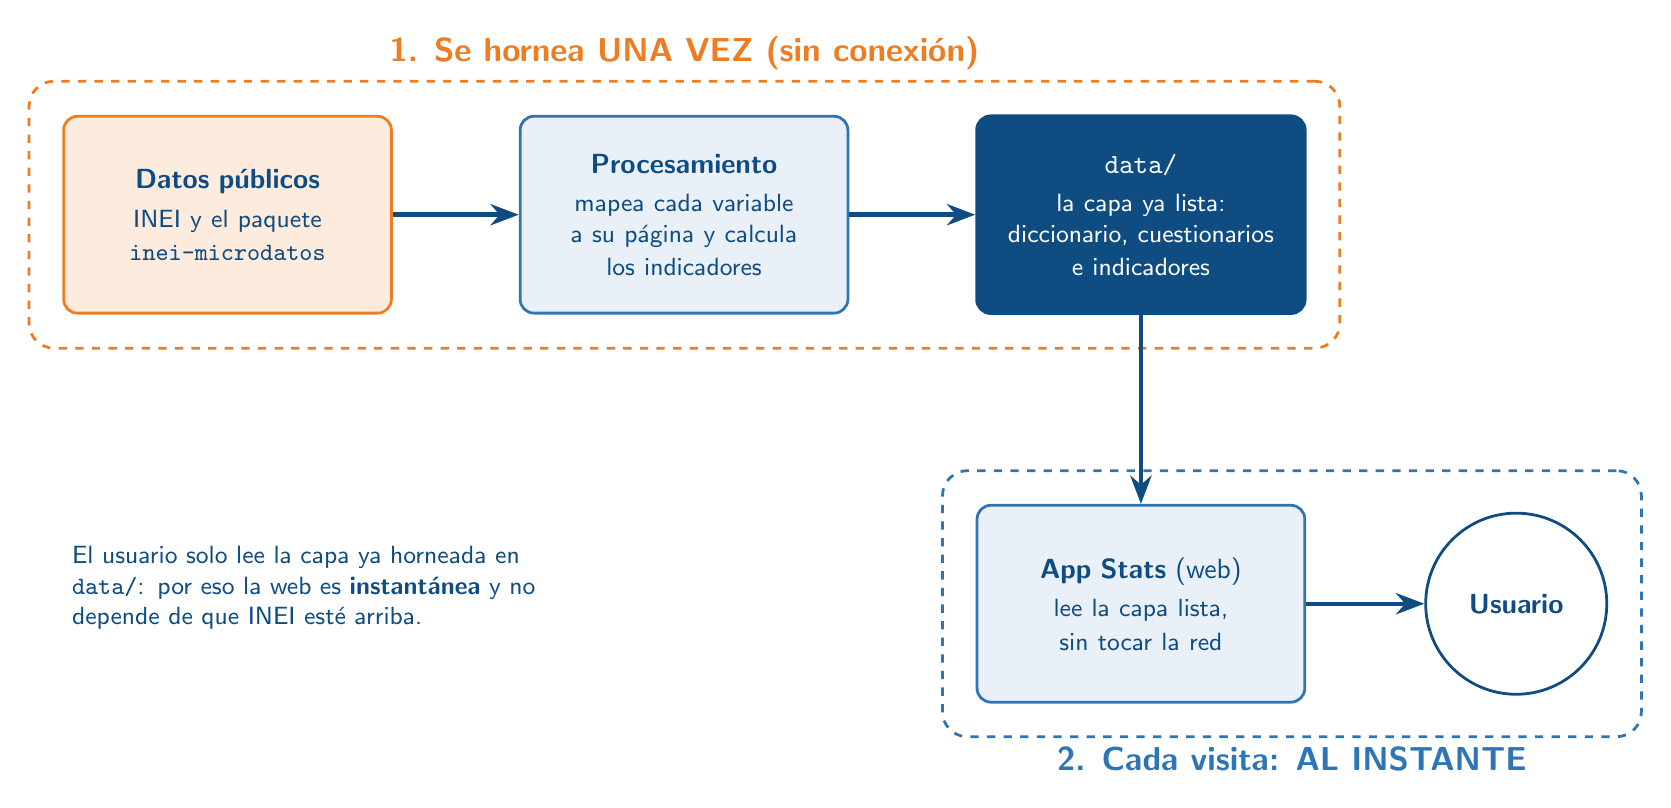
\begin{tikzpicture}[
  font=\sffamily,
  >={Stealth[length=3.6mm]},
  caja/.style={rounded corners=5pt, draw=AzulClaro, line width=1pt, fill=AzulSuave,
    text=AzulStats, align=center, inner sep=8pt, text width=3.6cm, minimum height=2.5cm},
  fuente/.style={rounded corners=5pt, draw=NaranjaStats, line width=1pt, fill=NaranjaSuave,
    text=AzulStats, align=center, inner sep=8pt, text width=3.6cm, minimum height=2.5cm},
  datos/.style={rounded corners=5pt, draw=AzulStats, line width=1.3pt, fill=AzulStats,
    text=white, align=center, inner sep=8pt, text width=3.6cm, minimum height=2.5cm},
  user/.style={circle, draw=AzulStats, line width=1pt, fill=white, text=AzulStats,
    align=center, inner sep=2pt, minimum size=2.3cm},
  flecha/.style={->, line width=1.6pt, AzulStats},
]

% --- Fila 1: se hornea una vez ---
\node[fuente] (src) {\textbf{Datos públicos}\\[3pt]\small INEI y el paquete\\ \texttt{inei-microdatos}};
\node[caja, right=16mm of src] (ai) {\textbf{Procesamiento}\\[3pt]\small mapea cada variable\\ a su página y calcula\\ los indicadores};
\node[datos, right=16mm of ai] (data) {\textbf{\texttt{data/}}\\[3pt]\small la capa ya lista:\\ diccionario, cuestionarios\\ e indicadores};

% --- Fila 2: cada visita ---
\node[caja, below=24mm of data] (app) {\textbf{App Stats} (web)\\[3pt]\small lee la capa lista,\\ sin tocar la red};
\node[user, right=15mm of app] (usr) {\textbf{Usuario}};

\draw[flecha] (src) -- (ai);
\draw[flecha] (ai) -- (data);
\draw[flecha] (data) -- (app);
\draw[flecha] (app) -- (usr);

% --- Bandas de fase ---
\begin{scope}[on background layer]
  \node[fit=(src)(data), draw=NaranjaStats, dashed, rounded corners=9pt, line width=1pt, inner sep=12pt,
    label={[NaranjaStats, font=\sffamily\bfseries\large]above:1. Se hornea UNA VEZ (sin conexión)}] {};
  \node[fit=(app)(usr), draw=AzulClaro, dashed, rounded corners=9pt, line width=1pt, inner sep=12pt,
    label={[AzulClaro, font=\sffamily\bfseries\large]below:2. Cada visita: AL INSTANTE}] {};
\end{scope}

% --- Nota en el hueco inferior izquierdo ---
\node[text width=6.4cm, align=left, font=\sffamily\small, text=AzulStats, anchor=west]
  at ([yshift=2mm]src.west |- app) {El usuario solo lee la capa ya horneada en \texttt{data/}: por eso
  la web es \textbf{instantánea} y no depende de que INEI esté arriba.};

\end{tikzpicture}
\end{document}
